% --------------------------------------|
% -------------------------------------|
% ------------------------------------|
\section{Investigación} 
% ------------------------------------\
% --------------------------------------\
% ----------------------------------------\

% INVESTIGAR Y RESPONDER AMPLIAMENTE

% --------------------------------------|
% -------------------------------------|
\begin{center}
    ¿Cuál es la diferencia entre Backtracking y el algoritmo de búsqueda BFS?
\end{center}
% --------------------------------------\
% ----------------------------------------\





% --------------------------------------|
% -------------------------------------|
\begin{center}
    ¿Cuál es la diferencia entre Backtracking y el algoritmo de búsqueda DFS?
\end{center}
\textbf{\large{Primero expliquemos que es el algoritmos DFS (Depth First Search):}}

Es un algoritmo utilizado en la teoría de grafos para buscar y recorrer grafos o árboles, no utiliza información sobre el costo de los movimientos o la ubicación de la meta.

El recorrido comienza revisando el nodo actual (la raíz si es un árbol o seleccionando un nodo arbitrario si no), después se mueve a uno de sus sucesores para repetir el proceso y explora tanto como sea posible en esa rama, si el nodo actual no tiene sucesor a revisar, regresamos a su predecesor y el proceso continua, es decir se mueve a otro sucesor del nodo, si la meta o solución es encontrada la búsqueda termina.

\begin{itemize}
    \item Pseudocódigo: El algoritmo DFS puede tener una implementación recursiva o iterativa (utilizando pilas), a continuación esta el pseudocodigo de la implementación recursiva:

    \begin{center}
        \begin{algorithmic}[1]
        \Procedure{DFS}{$\text{vertex } v$}
        \State $\text{visit}(v)$
        \ForAll{$\text{neighbor } u \text{ of } v$}
        \If{$u \text{ is undiscovered}$}
            \State $\text{call DFS}(u)$
        \EndIf
    \EndFor
\EndProcedure
        \end{algorithmic}
    \end{center}

    \item Gráfica: La siguiente gráfica muestra como se van descubriendo los nodos con el algoritmo DFS.

    \begin{center}
        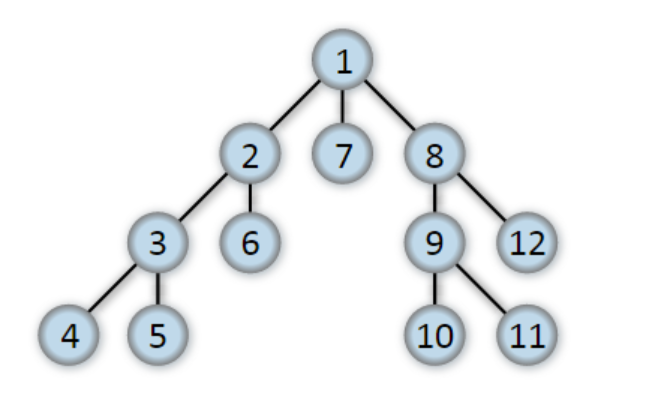
\includegraphics[scale = 0.5]{IMA/ejemploDFS.png}
    \end{center}

    \item Aplicaciones: Los principales usos que le dan al algoritmo son:
    \begin{itemize}
        \item Determinación de Conectividad: DFS se puede utilizar para determinar si un grafo es conexo, es decir, si hay un camino entre cada par de nodos.

        \item Detección de Ciclos: DFS puede detectar ciclos en un grafo no dirigido. Si mientras se ejecuta el algoritmo encuentra un nodo ya visitado, entonces hay un ciclo.

        \item Topological Sorting: DFS se puede utilizar para realizar una ordenación topológica en un grafo dirigido, que es una lista lineal de todos los nodos tal que para cada arista dirigida uv de un nodo u a un nodo v, u aparece antes que v en la lista.

        \item Encontrar Componentes Conectados: DFS se puede utilizar para encontrar los componentes conectados de un grafo no dirigido.

        \item Resolver acertijos con una sola solución, como laberintos.
    \end{itemize}

    \end{itemize}

Tiene una complejidad de O(n) en el peor de los casos y funciona mejor en árboles poco profundos.\\


    \textbf{\large{Diferencias entre DFS y Backtracking}}
    \\
    Ahora teniendo todo esto en cuenta la principal diferencia que tiene el \textbf{algoritmo DFS} con \textbf{backtracking} es que DFS encuentra una solución a un problema (ya que al encontrar una meta se deja de recorrer la gráfica) y backtracking encuentra todas las posibles soluciones de ese problema, entonces podemos decir que tienen diferencia en el espacio de búsqueda:
    \begin{itemize}
        \item DFS: Se adentra tanto como sea posible en la estructura del grafo antes de retroceder para explorar otras ramas.

        \item Backtracking: Explora todas las posibles soluciones de manera incremental, retrocediendo cuando se alcanza una solución inválida o se agotan todas las opciones.
    \end{itemize}

    Es decir el backtracking evalúa exhaustivamente cada posibilidad y retrocede cuando encuentra una solución inválida, mientras que DFS se adentra en la exploración del espacio de búsqueda, pero no garantiza encontrar todas las soluciones.

% --------------------------------------\
% ----------------------------------------\